\chapter{Kernfragestellung}

Die Kryptographie bzw. Verschlüsselung sind der Grundbaustein der IT-Sicherheit, der es ermöglicht, Dateien und Kommunikation vor unbefugten Zugriff zu schützen.
Seit Anbeginn des Computerzeitalters ist die konstante Suche und Entwickkung von immer komplexeren Verschlüsselungsmechanismen eine der Grundvoraussetzungen der Wahrung von digitalen Datensicherheit und sicherer Kommunikation. Die Notwendigkeit der stetigen Weiterentwicklung der Kryptographie, ergibt sich aus dem konstanten Wachstum der Rechenkapazität von Computern, welche sich in den letzten 50 Jahren aus den Fortschritten der Mikrochiptechnologie (in der Fachsspareche werden Mikrochips als Integrierte Schaltkreisebezeichnet) ergeben hat, siehe Abbildung \ref{fig:Bild0}.
\begin{figure}[htbp] 
  \centering
     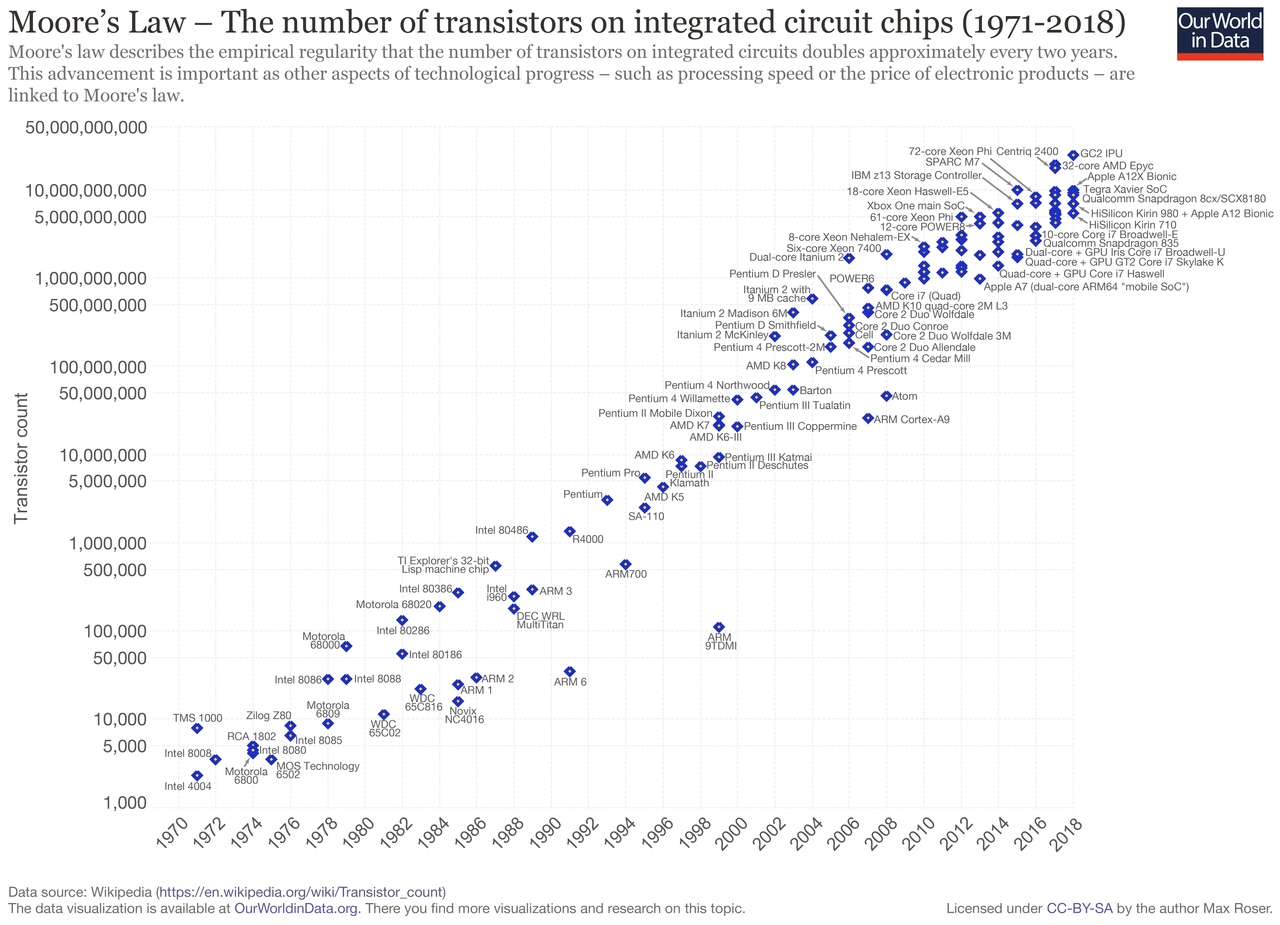
\includegraphics[width=0.9\textwidth]{img/Moores.png}
     \caption{Das mooresche Gesetz besagt, dass sich die Komplexität integrierter Schaltkreise alle 24 Monate verdoppelt.}
  \label{fig:Bild0}
\end{figure}
Die Komplexität hat sich über diesen Zeitraum ca. alle 24 Monate verdoppelt, dieser Trend wurde von Gordon Moore vorausgesagt und 1965 in einem Paper der Firma Intel erwähnt. Seine Aussage hat sich bewahrheitet und wurde in den Status der Gesetzmäßigkeit erhoben.
Mit der besagten Verdoppelung Komplexität geht eine Steigerung der Verarbeitungsleistung um den Faktor Wurzel aus 2 einher. (https://www.intel.de/content/www/de/de/it-managers/moores-law-evolution.html)

Mit einer gesteigerten Verarbeitungsleistung können bestehende Verschlüsselungen schneller entschlüsselt werden und werden dadurch unsicherer, weshalb diese also immer komplexer werden müssen um ein gewisses Niveau an Sicherheit garantieren zu können.
Diese Sicherheitsgarantie bezieht sich hauptsächlich auf den Aufwand, der betrieben werden muss um eine bestimmte Verschlüsselung aufheben zu können. Dieser Aufwan wird meistens in der Zeit gemessen die benötigt wird um eine bestimmte Verschlüsselung aufheben zu können.

Die Nutzung der Quantenmechanik für die Entwicklung von Computersystemen könnte in naher Zukunft eine Steigerung der Verarbeitungsleistung von Computersystemen erzielen, welche die bisherigen Entwicklungssteigerungen um ein vielfaches übertrifft.

Die bisherigen Entwicklungen der Quantencomputer haben bereits einen großteil der gängigen Verfahen obsolet gemacht obwohl sich die Technologie gewissermaßen noch in den Kinderschuhen befindet. Dies hat für die Forschung der Kryptographie das neue Zeitalter der \textbf{Post Quantum Cryptography} (\textbf{PQC})eingeleitet. Die \ac{PQC} hat mehrere Verfahren hervorgebracht, dessen Entschlüsselung eine mathematische Komplexität aufweisen, welche selbst für die extreme Verarbeitungsleistung von Quantencomputern eine große zeitliche Hürde bedeuten soll. Diese Verfahen sind jedoch bisher kaum praxiserprobt und müssen hinsichtlich der Sicherheit ihrer Implementierung noch weiter erforscht werden.Ein großer Unsicherheitsfaktor bleibt bei diesen Verhfahren die weitere Entwicklung des Quantencomputing, da diese sehr schwer einzuschätzen bleibt.[BSI1][BSI2] [Insert PQC Abkürzung]

In diesem Kontext können Verschlüsengsverfahren Abhilfe schaffen, welche sich ebenfalls die Prinzipien der Quantenphysik zu nutze machen, dieses Vorgehen wird als Quantenkryptographie bezeichnet. Der Ansatz der im Rahmen dieses Forschungsprojekts erprobt werden soll nennt sich \textbf{Quantum Key distribution} (kurz \ac{QKD}).